\documentclass[11pt,a4paper]{article}

\usepackage[czech, english]{babel}
\usepackage[T1]{fontenc}
\usepackage[utf8]{inputenc}

\usepackage[square, numbers]{natbib} % sazba pouzite literatury
\usepackage{indentfirst} % 1. odstavec jako v cestine, pro práci v aj možno zakomentovat
\usepackage{fancyhdr} % tisk hlaviček a patiček stránek
\usepackage{nomencl} % umožňuje snadno definovat zkratky a jejich seznam

% \usepackage{lmodern}
\usepackage{graphicx}
\usepackage{caption}
\usepackage{subcaption}
\usepackage{xspace}
\usepackage{enumerate}
\usepackage{enumitem}
\usepackage{bbding}
\usepackage[usenames,dvipsnames]{color} % barvy
\usepackage{url}
\usepackage{subscript}

\usepackage{tabularx}
\usepackage{pdflscape}
\usepackage{lipsum}

\usepackage{courier}
\usepackage{float}
\usepackage{nonfloat}
\usepackage{wrapfig}

% utrzky kodu
\usepackage{listings,xcolor}
\usepackage{inconsolata}
\usepackage{algorithm}
\usepackage{algorithmicx} %slouží pro zápis algoritmů
\usepackage{algpseudocode} %slouží pro výpis pseudokódu
\usepackage{eqparbox}
\usepackage{dirtree}
\usepackage{array}
\usepackage{amsmath} % matematicke symboly
\usepackage{amsfonts}
\usepackage{amsxtra} % matematicka pismena
\usepackage{wasysym} % znak vyplnene sipky
\usepackage{setspace} % vyska radku
\usepackage{changepage} % zmena okraju stranky
\usepackage{soul}
\usepackage{datetime} % datum a cas
\usepackage{tabu} % vylepsene tabulky - ruzne siroke ohraniceni
\usepackage{pgfgantt}
\usepackage{textcomp}
\usepackage{pgfplots}
\usepackage{filecontents}
\usepackage{pgfplots}
\usepackage{tikz} % grafy
\usetikzlibrary{arrows,shapes,backgrounds,snakes,patterns,calc,trees,positioning,chains,shapes.geometric,decorations.pathreplacing,decorations.pathmorphing,matrix,shapes.symbols,pgfplots.groupplots}

% custom packages
\usepackage{_lib/infodata} % info strings
\usepackage{_lib/mathstyle}
\usepackage{_lib/macros}
\usepackage{_lib/colors} % barvy
\usepackage{_lib/codestyle} % highlight zdrojovych kodu
\usepackage{_lib/mathstyle} % matematicke pomocne fce

\usepackage{_lib/qtree}

\begin{document}
    \selectlanguage{czech}

    %%  Titulni strana  %%
    \rendercoverpage

    %%  Obsah  %%
    \tableofcontents
    % smazani cisla stranky u obsahu
    \addtocontents{toc}{\protect\thispagestyle{empty}}

    \rendermainbody

    %!TEX root=../oi-magistr-si.tex
\section[TPJ - sémantiky: operační, denotační]{Sémantika: operační sémantika, denotační sémantika, pevný bod funkce, vázání jmen, stav programu a data.}

\noindent Sémantika programovacích jazyků je v teorii programovacích jazyků \textbf{obor} zabývající se \textbf{důsledným matematickým popisem významu} programovacího jazyka \cite{wiki:semantika}.

\noindent 3 hlavní charakteristiky jazyka jsou: 

\begin{itemize}[itemsep=0px]
\item \textbf{syntaxe} se zabývá formou (znaky a jejich vztahy),
\item \textbf{sémantika} významem znaků,
\item \textbf{pragmatika} závislostí konstrukcí na nositeli - implementace.
\end{itemize}

\textbf{Operační sémantika} je \textbf{přístup}, který \textbf{definuje sémantiku} programovacího jazyka tak, že určí jak je libovolný program vykonán na počítači, jehož činnost je známa. Může to být nějaký abstraktní stroj, který je dostatečně jednoduchý pro snadné pochopení jeho činnosti (například Turingův stroj). Operační sémantika potom specifikuje, jak tento stroj zpracovává program v definovaném jazyku.

\paragraph{Operační exekuce}

\begin{itemize}[itemsep=0px]
\item Program + vstupy $\rightarrow$ Vstupní funkce
\item Iniciální konfigurace
\item (Mezikonfigurace ...)
\item Finalní konfigurace
\item Výstupní funkce $\rightarrow$ Odpověď
\end{itemize}

\subsection{Sémantika malého kroku (SOS)}
\begin{itemize}[itemsep=0px]
\item Definujeme přepisovací relaci $\Rightarrow \in Expr \times Expr$.
\item Výraz $e \Rightarrow e'$ znamená, že přepis $e$ na $e'$ je vykonán v jednom kroku.
\end{itemize}

\paragraph{Formální definice} $S = \langle CF,\Rightarrow, FC, IF, OF \rangle$

\begin{itemize}[itemsep=0px]
\item CF – doména konfigurací (obor hodnot)
\item $\Rightarrow$ – přepisovací relace (transformuje konfigurace) ($\Rightarrow \subseteq CF \times CF$)
\item FC – množina finálních konfigurací (nezjednodušitelné konfigurace) ($FC\subseteq CF$)
\item IF – vstupní funkce $(\text{Prog} \times \text{Inputs}) \rightarrow CF$.
\item OF – výstupní funkce $FC \rightarrow \text{Answer}$
\end{itemize}

\paragraph{Pravidla} $e,e_1,e_2,e' \in Expr \quad n,n' \in Num$

$$\frac{}{\bigtriangleup n \Rightarrow -n}$$

$$\frac{}{n \odot n' \Rightarrow n + n'}$$

$$\frac{e \Rightarrow e'}{e \bigtriangleup \Rightarrow \bigtriangleup e'}$$

$$\frac{e_1 \Rightarrow e'}{e_1 \odot e_2 \Rightarrow e' \odot e_2}$$

$$\frac{e_2 \Rightarrow e'}{e_1 \odot e_2 \Rightarrow e_1 \odot e'}$$

\subsection{Sémantika velkého kroku (BOS)}
\noindent Odlišný přístup než SOS. Program je vyhodnocen v jednom kroku. Zde je definována přepisovací relace

$$\Longrightarrow \in Expr \times Num$$

\paragraph{Pravidla} $e,e_1,e_2 \in Expr \quad n,n_1,n_2 \in Num$

$$\frac{}{n \Longrightarrow n}$$

$$\frac{e \Longrightarrow n}{\bigtriangleup e \Longrightarrow -n}$$

$$\frac{e_1 \Longrightarrow n_1 \quad e_2 \Longrightarrow n_2}{e_1 \odot e_2 \Longrightarrow n_1 + n_2}$$

\example{Příklad SOS (jedno z možných vyhodnocení):}{
    \begin{spacing}{0}
    $$
    \cfrac{
        \cfrac{
            \cfrac{}{
                \bigtriangleup 15 \Rightarrow -15
            }
        }{
        (\bigtriangleup 15) \odot (\bigtriangleup 24) \Rightarrow -15 \odot (\bigtriangleup 24)
        }
    }{
        \bigtriangleup((\bigtriangleup 15) \odot (\bigtriangleup 24)) \Rightarrow \bigtriangleup(-15 \odot (\bigtriangleup 24))
    }$$
    \end{spacing}
    \vspace{20px}
}

\example{Příklad BOS:}{
    \begin{spacing}{0}
    $$
    \cfrac{
        \cfrac{
            \cfrac{
                \cfrac{}{
                    15 \Longrightarrow 15 \quad 24 \Longrightarrow 24
                }
            }{
                \bigtriangleup 15 \Longrightarrow -15 \quad \bigtriangleup 24 \Longrightarrow -24
            }
        }{
        (\bigtriangleup 15) \odot (\bigtriangleup 24) \Longrightarrow -15 + -24
        }
    }{
        \bigtriangleup((\bigtriangleup 15) \odot (\bigtriangleup 24)) \Longrightarrow -(-15 + -24)
    }$$
    \end{spacing}
    \vspace{20px}
}



\subsection{Denotační sémantika}

Denotační sémantika používá k popisu sémantiky programovacího jazyka funkce. Tyto funkce přiřazují sémantické hodnoty správným syntaktickým zápisům. Příkladem může být funkce Val, která přiřadí výrazu jeho hodnotu:

$$\text{Val}: \text{Výraz} \rightarrow \text{Integer}$$

Doménou syntaktických funkcí se nazývá syntaktická doména - u funkce Val je to množina všech správných aritmetických výrazů. Obor hodnot je sémantická doména - zde množina celých čísel. Denotační definice jazyka má tedy 3 části - syntaktickou doménu, sémantickou doménu a definici jednotlivých funkcí.

\begin{itemize}[itemsep=0px]
\item \textbf{Syntaktická algebra} - popisuje abstraktní syntaxy jazyka, může být specifikována gramatikou.
\item \textbf{Sémantická algebra} - modeluje význam frází, skládá se z kolekce sémantických domén.
\item \textbf{Významová funkce} - mapuje elementy syntaktické algebry k jejich významu v sémantické algebře. Funkce musí být homomorfismus mezi syntaktickou a sémantickou algebrou.
\end{itemize}

\subsubsection{Významová funkce (Meaning function)}
Uvažujte $M$ jako významovou funkci a $t$ je prvek v abstraktním syntaktickém stromu s potomky $t_1, \hdots, t_k$. Pak

$$(M t) = (f_t (M t_1) \hdots (M t_k))$$

kde $f_t$ je funkce určená syntaktickou třídou.

\begin{figure}[h!]
\centering
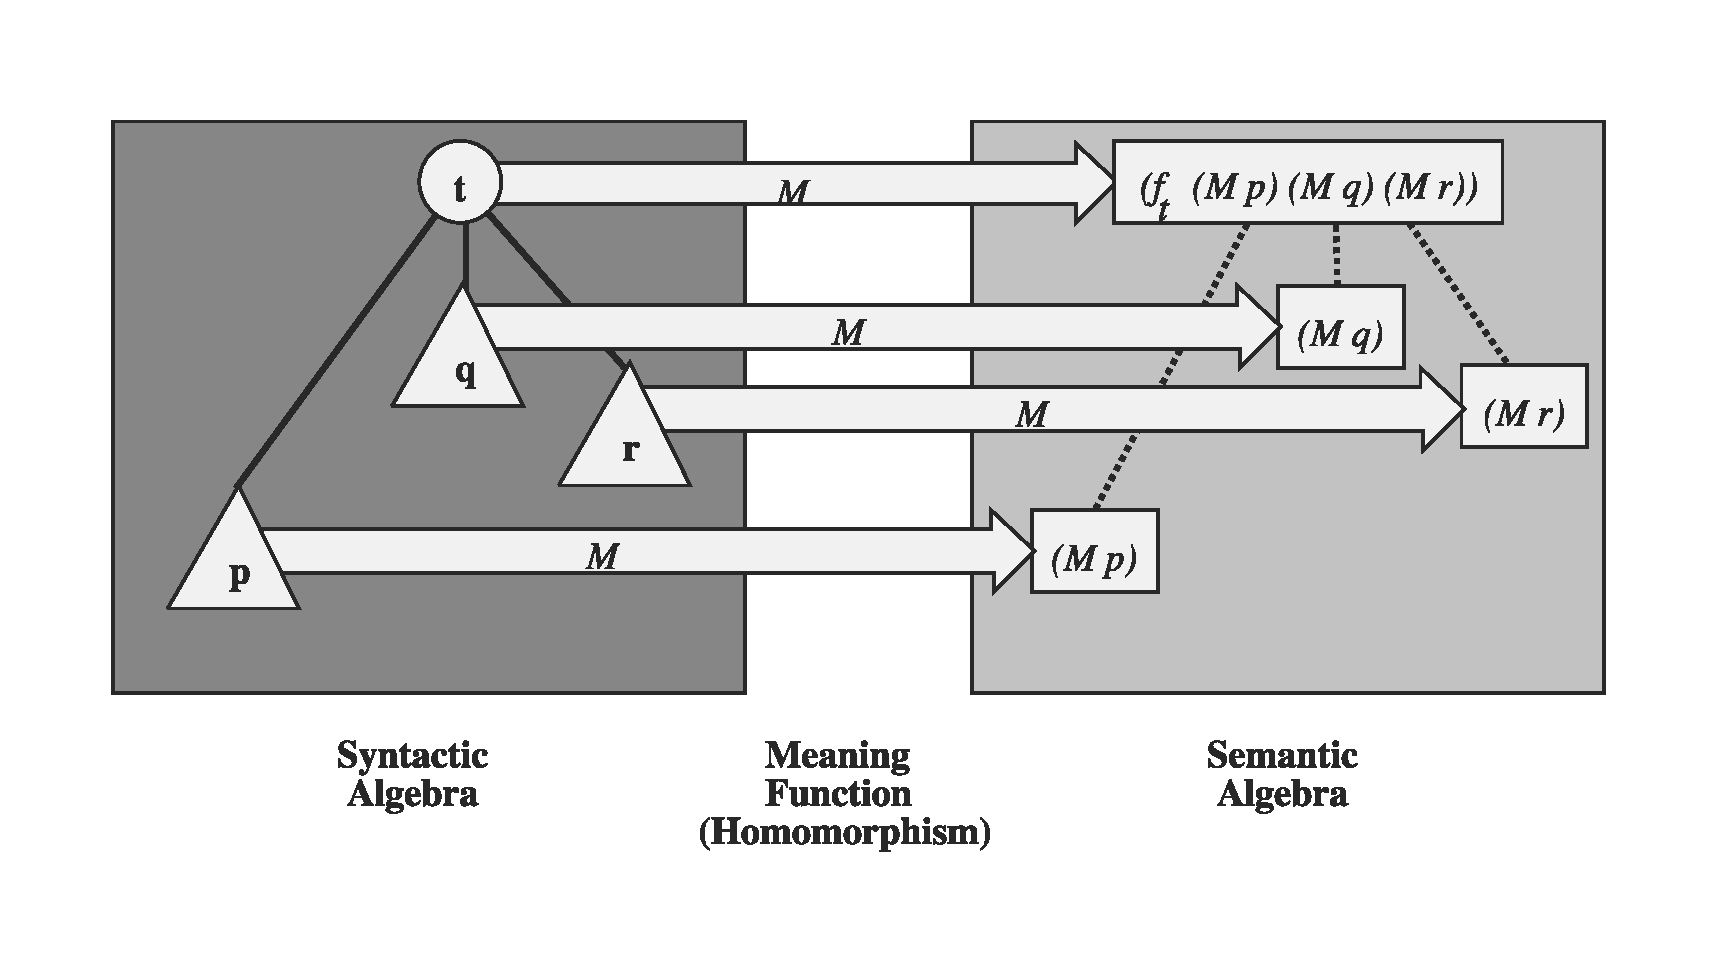
\includegraphics[width=125mm]{01/images/tpj-homo}
\end{figure}

\paragraph{Denotační sémantika} $Expr $ ::= $ Num \quad | \quad \bigtriangleup Expr \quad | \quad Expr \odot Expr$

\noindent Sémantická doména $N$

$$[\![n]\!] = n$$

$$[\![\bigtriangleup e]\!] = [\![\bigtriangleup]\!]([\![e]\!])$$

$$[\![\bigtriangleup]\!] = \lambda x.-x \quad \text{(např. unární mínus)}$$

$$[\![e_1 \odot e_2]\!] = [\![\odot]\!]([\![e_1]\!], [\![e_2]\!])$$

$$[\![\odot]\!] = \lambda x,y.x+y \quad \text{(např. plus)}$$

\subsection{Pevný bod funkce}
Jako pevný bod označujeme bod, který se v daném zobrazení zobrazí sám na sebe. Označuje se také jako samodružný bod. Například pevnými body funkce $f(x)=x^2-4x+6$, jsou čísla 2 a 3.

\begin{itemize}
\item bod, ve kterém platí $f(x) = x$
\item využívá se pro rekurzivní funkce
\item Y kombinátor v lambda kalkulu: \texttt{Y = $\lambda$y($\lambda$x.y(xx))($\lambda$x.y(xx))}
\end{itemize}

\priklad
Generující funkce faktoriálu fact = \texttt{$\lambda$F.$\lambda$X.if x==0 then 1 else F(decrement(X))}. Generující funkci dám do Y kombinátoru:

\begin{lstlisting}[
  mathescape,
  columns=fullflexible,
  basicstyle=\fontfamily{lmvtt}\selectfont,
]
Y fact =
       = $\lambda$f ($\lambda$x.y(xx))($\lambda$x.y(xx)) fact =
       = ($\lambda$x.fact(xx))($\lambda$x.fact(xx)) =
       = fact( ($\lambda$x.fact(xx) ($\lambda$x.fact(xx) ) =
       = fact(Y fact)
\end{lstlisting}

\noindent \texttt{Y fact} je pevný bod funkce, která počítá faktoriál.

\subsection{Vázání jmen}
Vázání jmen se vyskytuje v lambda kalkulu.
\paragraph{$\lambda$-kalkul} Je formální popis, který slouží jako základ pro funkcionální jazyky, takže všechny konstrukce v těchto jazycích jdou přepsat právě na $\lambda$-kalkul. Základní prvky $\lambda$-kalkulu jsou tři následující:
\begin{itemize}
\item \textbf{Proměnné} Obyčejné proměnné, tak jak je znáte z jiných jazyků, většinou se značí \texttt{x,y,z}.

\item \textbf{Abstrakce} Definice funkce – představte si např. funkci \texttt{f(x) = x+2}, tak přesně taková funkce se v $\lambda$-kalkulu zapíše takto: \texttt{$\lambda$x.x+2}. Část mezi $\lambda$ a tečkou jsou parametry funkce (zde máme pouze jeden parametr) a za tečkou se nachází tělo funkce.

\item \textbf{Aplikace} Volání funkce – když si vezmu naši funkci \texttt{f(x) = x+2}, tak ta se zavolá např. s argumentem 3 takto: \texttt{f(3)}. Funkce v $\lambda$-kalkulu se volají podobně, funkce se volá takto: \texttt{(f 3)}, tzn. nejdříve je uvedena funkce a poté její argumenty. Funkce f se v $\lambda$-kalkulu tedy zavolá takto: \texttt{($\lambda$x.x+2) 3}. Vysvětlení by mělo být už jasnější. Číslo 3 se dosadí za parametr \texttt{x} a přejde se do těla funkce, tam se ke 3 přičte 2 a výsledkem je 5.
\end{itemize}

\noindent Proměnná je v $\lambda$-výrazu \textit{vázaná}, pokud se jedná o parametr nějaké funkce, takže např. ve výrazu (\texttt{$\lambda$x.yx}) je \texttt{x} vázaná proměnná. Ostatní proměnné (v minulém příkladu \texttt{y}) jsou \textit{volné}. Proměnná se vždycky váže na nejbližsí lambdu vlevo, takže ve výrazu \texttt{($\lambda$x(($\lambda$x.x) w))} se proměnná \texttt{x} uprostřed výrazu váže na lambdu co je hned vlevo od ní a ne na tu úplně vlevo! Proměnná \texttt{w} je samozřejmě volná \cite{lambda}.

\begin{itemize}
\item Funkce, co mají jen vázané proměnné, vrátí při každém zavolání stejný výsledek. Funkce s volnými proměnnými jsou závislé na globálním kontextu.
\item Funkce, co mají jen vázané proměnné, se v $\lambda$-kalkulu nazývají kombinátory.
\end{itemize}

$$\texttt{(}\lambda\texttt{x.xy)}$$

$$\texttt{(}\lambda\texttt{x.x)(}\lambda\texttt{y.yx)}$$

\subsection{Stav programu}
Stav = proměnné v prostředí, proměnné mají typ, prostředí = množina všech proměnných, kontext (v handoutech $\Gamma$ (Gamma))
Čistě funkční jazyky (a matematika) jsou bezestavové, stavové výpočty mohou být reprezentovány jako iterace skrz stavy.

Čistě funkční jazyky (a matematika) jsou bezestavové, stav může být modelován jako iterace skrz stavy.
\example{Funkce na nalezení maxima z pole:}{
$$max:N* \rightarrow N$$

$$max(\langle a_1, \hdots, a_n \rangle) = loop(\langle a_1, \hdots, a_n \rangle,1,0)$$

$$loop: N* \times N \times N \rightarrow N$$

$$loop(\langle a_1, \hdots, a_n \rangle,c,m) = m \qquad \text{if} \quad c > n$$

$$loop(\langle a_1, \hdots, a_n \rangle,c,m) = loop(\langle a_1, \hdots, a_n \rangle,c+1,m) \qquad \text{if} \quad c \leq n \wedge a_c \leq m$$

$$loop(\langle a_1, \hdots, a_n \rangle,c,m) = loop(\langle a_1, \hdots, a_n \rangle,c+1,a_c) \qquad \text{otherwise}$$

\vspace{20px}
}

\paragraph{Monády} - struktury (typy), co reprezentují výpočet jako sekvenci kroků.

\subsection{Data programu}
Dělí se na \textbf{součiny}, \textbf{sumy} a \textbf{sumy součinů}.

\begin{itemize}[itemsep=0px]
\item Součiny
\begin{itemize}[itemsep=0px]
\item Positional data = N-tice, každý prvek může mít jiný typ
\item Sequence, List = pole
\item Named = třída
\item Nonstrict, stream = data, která se získají/vypočítají v okamžiku, kdy je potřeba (např. InputStream, odněkud se to vezme)
\end{itemize}

\item Sumy - Union v C, nadtypy v Javě.
\item Sumy součinů - Binární a ternální operátory, double dispatch.
\end{itemize} % TPJ
    %!TEX root=../oi-magistr-si.tex
\section[TPJ - Statická sémantika]{Statická sémantika: typy, polymorfní typy, typy vyššího řádu, rekonstrukce (inference) typů, abstraktní typy.}

Statická sémantika je řešena při překladu programu, zde jsou definovány a deklarovány jednotlivá pravidla a prvky programovacího jazyka. V těchto prvcích je zahrnuta jazyková konstrukce, její typy parametrů, význam příkazů a další prvky. Statická sémantika dále kontroluje statické typy a práci s tabulkou definovaných programových symbolů.

\begin{itemize}[itemsep=0px]
\item Staticky typované jazyky požadují uvedení datového typu u každé deklarace. Zde nelze deklarovat proměnnou, či funkci nebo objekt bez zadání datového typu.
\item Všechny typové kontroly jsou prováděny staticky při překladu. Už při překladu má být každé proměnné přiřazen datový typ.
\item Je možné daný datový typ přímo přetypovat. Přetypování především slouží k obcházení typových kontrol.
\item \textbf{Výhodou statického typování je lepší možnost odhalení typových chyb.}
\item Hlavní nevýhodou této metody je větší složitost programových konstrukcí, délka zdrojového kódu a tím i menší pružnost programovacího jazyka.
\item K nejčastěji vyskytovaným běhovým chybám patří přetečení datového typu.
\item Mezi neznámější zástupce staticky typovaných jazyků patří Java, Ada a jazyk C.
\end{itemize}

\subsection{Typy}

$$\Gamma \vdash e : A \qquad \text{\uv{$e$ je well-formed term typu $A$ v prostředí $\Gamma$}}$$

\begin{itemize}[itemsep=0px]
\item Typování
\begin{itemize}
\item \textbf{statické} - formálně specifikováno typovým systémem (judgements, typová pravidla, prostředí). Typová pravidla rozhodují platnost rozhodnutí (judgements) na základě jiných rozhodnutí o kterých je známo, že jsou platné.
\item \textbf{dynamické}
\end{itemize}
\item Typ je množina přípustných hodnot a operací s nimi.
\item \textbf{TopType}
\item \textbf{Type preservation} - zachování typu během přepisovací relace $\forall e,e'\in Expr:(\vdash e:t) \wedge e \rightsquigarrow e' \Rightarrow (\vdash e':t)$
\item \textbf{Progress} - když mám nějaký term v konfiguraci, tak pak to je buď finální konfigurace, nebo lze ještě nejméně jednou přepsat. Tzn. dobře otypovaný term neskončí ve \textit{stuck} stavu (stav, pro který není definován výstup). (důkaz lze udělat analýzou pravidel). $\forall e \in Expr: (\vdash e:t) \Rightarrow e \in (Num \cup Bool) \vee \exists e' \in Expr: e \rightsquigarrow e'$.
\item Type preservation + progress = \textbf{Soundness}. An argument is sound if and only if: \textit{The argument is valid} and \textit{All of its premises are true}. (i.e. All men are mortal. Socrates is a man. Therefore, Socrates is mortal.)
\item \textbf{Terminace} - důkaz např pomocí \textit{energie}, nadefinuji \uv{energii}, nadefinuji, že při každém přepsání se musí snížit.
\item \textbf{Determinismus} - programovací jazyk je deterministický právě tehdy když existuje právě jeden výstup pro každý pár \textit{programu} a \textit{vstupů}.
$\forall v,v' \in (Num \cup Bool): \forall e \in Expr : e \rightsquigarrow^* v \wedge e \rightsquigarrow^* v' \Rightarrow v = v'$. Platí to, protože platí konfluence relace.
\item \textbf{Konfluence} - \uv{strom vyhodnocování relace se rozdělí a pak se zase spojí}.
\end{itemize}

\subsection{Polymorfní typy}
Polymorfní typ je typ, jehož operace mohou být aplikovány na hodnoty jiného typu.
\begin{itemize}
\item \textbf{Rekurzivní} - používají se na zakodování seznamů a stromů, obsahují více hodnot stejného typu \url{http://en.wikipedia.org/wiki/Recursive_data_type}
\item \textbf{Univerzální} - generický typ, např. List<X>
\item \textbf{parametrický polymorfismus} - pomocí něj lze zapsat funkce jedním stylem a zároveň zachovat bezpečné typování. Tzn. funkce je zapsána genericky a umí zpracovávat vstupy bez ohledu na jejich typ. Typický příklad je třeba funkce append která se může zavolat s jakýmkoliv typem a správně se vyhodnotí. Není potřeba deklarovat \texttt{append :Integer} nebo \texttt{append:Bool}.
\item \textbf{ad-hoc polymorfismus} - jedna funkce může mít mnoho implementací na základě zpracování jednotlivých typů - přetěžování funkcí v Javě.
\end{itemize}



\subsection{Typy vyššího řádu}
\begin{itemize}
\item Product Type - např. tuple, 2 a více typů, 2 operandy ($A \times B$) \url{http://en.wikipedia.org/wiki/Product_type}
\item Union Type - datová struktura, která může udržovat více fixních typů \url{http://en.wikipedia.org/wiki/Tagged_union}
\item Function Type
\item Record Type - klasický objekt, který má fieldy
\end{itemize}

Jde o takzvané monády a debuggable functions (tohle je spíš možné využití). 

\paragraph{Monády} - umožňují řetězit procedury za pomocí čistě funkcionálního programování. Skládají se ze dvou operací a to bind a return(unit). 

\noindent \textit{\uv{In functional programming, a monad is a structure that represents computations defined as sequences of steps: a type with a monad structure defines what it means to chain operations, or nest functions of that type together. This allows the programmer to build pipelines that process data in steps, in which each action is decorated with additional processing rules provided by the monad.}}


\subsection{Rekonstrukce typů}
Schopnost z proměnné vyvodit její typ. Je to vlastnost některých silně staticky typovaných jazyků.

\noindent \textit{\uv{Type inference refers to the automatic deduction of the data type of an expression in a programming language. If some, but not all, type annotations are already present it is referred to as type reconstruction.}}

Například v csharpu, stačí místo typu psát klíčové slovo \texttt{var}.

\begin{verbatim}
var results = new Car();
// results je typu Car
\end{verbatim}

\subsection{Abstraktní typy}
Příkladem jsou Abstraktní třídy v Javě. Vyskytují se hlavně ve staticky typovaných jazycích.

Fronta, HashMapa, Množina (Set), Seznam (List), Zásobník (Stack), ...
 % TPJ
    %!TEX root=../oi-magistr-si.tex
\section[NUR - Teorie HCI]{Teorie HCI, kognitivní aspekty, způsoby interakce, speciální uživatelská rozhraní.}
\subsection{HCI - Human-Computer Interaction}

Human-Computer Interaction (česky interakce člověk - počítač) je průnikový \textbf{obor, který se zabývá fenoménem tvorby UI}. Zabývá se analýzou návrhu, vyhodnocování a zavádění interaktivních výpočetních systémů používaných lidmi a jevů, které interakci doprovázejí. Skládá se ze tří částí: \textbf{jedinec, počítač a způsob, jakým dohromady spolupracují}.

Cílem je návrh a vývoj prostředků a systémů, které jsou použitelné, efektivní, bezpečné a intuitivní. Dále se snaží přizpůsobit výměnu dat mezi lidmi a stroji tak, aby byla méně stresující a náchylná k nedorozumění.

\subsection{Kognitivní aspekty}
\begin{itemize}[itemsep=0px]
\item \textbf{kognitivní psychologie} zkoumá proces myšlení, učení a rozhodování
\item mentální model:
    \begin{itemize}[itemsep=0px]
    \item kognitivní struktura
    \item vnitřní reprezentace okolního světa, kterou si vytváříme v hlavě
    \item jak objekty určité třídy reagují s objekty jiné třídy, jak objekty v průběhu interakce mění své vlastnosti
    \item založeny na zkušenosti, mohou být nepřesné, neodpovídat zákonům fyziky
    \item lze je použít k predikci (kam dopadne hozený míč)
    \end{itemize}
\item kognitivní model uživatele - model, jak uživatel pracuje, na jehož základě se předpoví jeho chování (interakce s UI), výhody: nemusí se vytvářet prototypy, není nutné testování se skutečnými uživateli, vědecký základ pro návrh
\item estetika a efektivita kognitivních funkcí - důležitost vizuální podoby, atraktivní věci jsou použitelnější
\end{itemize}

\paragraph{Kognitivní teorie v HCI}
Modelování úkolů - metody KLM, GOMS
\begin{itemize}[itemsep=0px]
\item GOMS (Goals, Operators, Methods, Selectors) - popis struktury úloh, task rozpadlý do menších subtasků v hierarchicky přehledné síti,expert provádí UI operace
\item KLM (Keystroke-Level Model) - low-level verze GOMS, uživatelské operátory (K-keystroke, P-point, D-drawing, M-mental think), tabulkové časy pro každý operátor, každé operaci se přiřadí čas vykonání
\item Hick's Law - čas potřebný k rozhodnutí se, $n$ stejně pravděpodobných možností, průměrný čas výběru jedné z nich: $T = b \log_2(n + 1)$
\item Fitt's Law - předpovídá jak dlouho trvá uživateli vybrat cíl, vyhodnocení vstupních zařízení, pohyb k cíli o velikosti S ve vzdálenosti D: $T = a + b \log (\frac{D}{S} + 1)$, $a, b$ - konstanty závislé na zařízení
\item Model Human Processor / Human Information Processor Model - model lidského poznání vytvořený za použití teorií uvedených výše, modeluje, jak uživatel zachází s informacemi, perceptuální, kognitivní a motorický subsystém
\end{itemize}

\subsection{Způsoby interakce}
\begin{itemize}[itemsep=0px]
\item přímá manipulace - hry (značné implementační požadavky)
\item navigace (menu, odkazy) - web - není třeba si pamatovat příkazy jako CL, ale zabírá příliš místa na obrazovce
\item formuláře - web
\item příkazy - unix, první metoda komunikace člověk - PC, BNF, konečný automat
\item přirozený jazyk
\item nové typy interakce - mluva, gesta, eye-tracking, haptické (hmatová odezva) displeje
\end{itemize}

\subsection{Speciální UI}
\begin{itemize}[itemsep=0px]
\item mluvící systémy AI (Eliza, Cortana, Siri atd.)
\item multimodální - kombinování více vstupů
\item pokročilý vstup z klávesnice - pubtran se \uv{učí}
\item magnetický prsten - klikání, scrollování
\item haptická odezva
\item papírový mobil - ohýbací gesta
\item spolupráce telefonů např při sharování
\item multi-touch
\end{itemize}


\paragraph{Architektura UI}
Cíl: oddělení UI a aplikace, výběr možností prezentace informace uživateli, koordinace interakce, modifikovatelnost a přenositelnost. Interaktivní systém poskytuje tři funkce (vrstvy):
\begin{itemize}[itemsep=0px]
\item prezentační (UI)
\item dialogovou (komunikace s uživatelem)
\item aplikační (vlastní účel SW systému)
\end{itemize}
\textbf{Monolická architektura} = všechny části v jednom

\paragraph{Seeheim model}
\href{http://centurion2.com/SEHomework/UserInterfaceDesign/UserInterfaceDesign.php#SeeheimModel}{URL}
sémantická vazba je často pomalejší, přímá vazba mezi aplikační a prezentační vrstvou regulovaná dialogem umožní okamžitou odezvu (switch).

Výhody:oddělená prezentační vrstva podporuje přenositelnost a modifikovatelnost, oddělená aplikační vrstva dovoluje modifikace aplikace beze změny UI, oddělená dialogová část umožňuje změnit uživatelskou interakci beze změny prezentační části.
Nevýhody: řada modifikací se promítá do všech částí, komplikované sémantické vazby.

$$lexical \qquad - \qquad syntactic \qquad - \qquad semantic$$
$$\text{Prezentace} \qquad - \qquad \text{Dialog} \qquad - \qquad \text{Aplikace}$$ % NUR
    %!TEX root=../oi-magistr-si.tex
\section[NUR - Metody návrhu, uživatelské a konceptuální modely]{Metody návrhu, uživatelské a konceptuální modely}

\begin{figure}[h!]
\centering
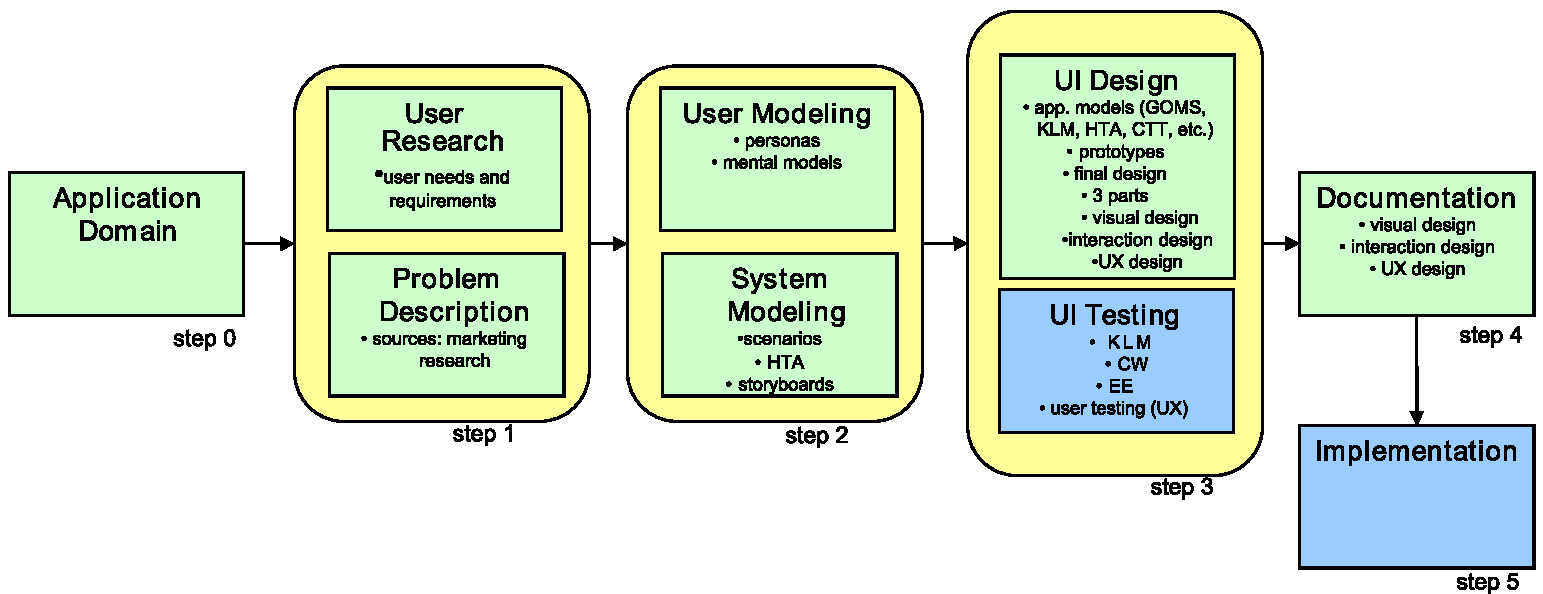
\includegraphics[width=125mm]{04/images/hci}
\end{figure}

\paragraph{Cyklus tvorby UI}
\begin{itemize}[itemsep=0px]
\item Návrh - porozumění uživateli (cílová skupina) a jeho potřebám
\begin{itemize}[itemsep=0px]
\item \textbf{analýza úlohy} - výkonnost software, hardware, uživatele při provádění úlohy, co uživatelé dělají, co k tomu potřebují za nástroje, co potřebují vědět, metoda: HTA
\item popis průběhu dialogu, slouží k následující implementaci UI
\end{itemize}
\item Implementace - prototypování
\item Vyhodnocení - hodnocení prototypu ve spolupráci s uživateli (kvalitativní \&
kvantitativní)
\item další iterace...
\end{itemize}

\paragraph{Analýza}
\begin{itemize}[itemsep=0px]
\item specifikace aktivit, které systém bude dělat
\item specifikace uživatelů - ti, kteří aktivity budou dělat
\item volba formy řešení - forma UI, SW podporující UI, OS, systémové požadavky, HW
\end{itemize}

\paragraph{Uživatel}
\begin{itemize}[itemsep=0px]
\item Uživatelské požadavky - Obecné požadavky: fyzické, kognitivní, sociální. Mohou být také specifické požadavky, které se vztahují přímo k problémmu.
\item Modely uživatele - KLM (Keystroke-level model), persony
\end{itemize}

\paragraph{Principy použitelného návrhu (usable design)}
\begin{itemize}[itemsep=0px]
\item jednoduché a přirozené dialogy v jazyku uživatele
\item konzistentnost akcí, příkazu, layoutu, terminologie
\item minimalizovat paměťovou zátěž uživatele - rozpoznávání je snazší než
vzpomínání
\item zpětná vazba
\item kontrola vstupu
\item snadné vrácení akcí - podpoří chuť experimentovat
\item výrazně značená ukončení - uživatel se nesmí ocitnout v pasti
\item zkratky - rychlé provedení časté akce pro zkušené uživatele
\item robustní systém poskytující snadno ovladatelné prostředky k nápravě chyb
\item užitečná nápověda a dobrá dokumentace (hledána v kritických situacích)
\end{itemize}

\paragraph{Terminologie}
\begin{itemize}[itemsep=0px]
\item Goal - to čeho chceme dosáhnout
\item Task - posloupnost aktivit, která dá \textit{goal}
\item Action - krok nebo akce - část \textit{tasku}
\end{itemize}

\subsection{Specifikace požadavků}
\begin{itemize}[itemsep=0px]
\item HTA (Hierarchical task analysis) - dekompoziční strom, kde je \textit{goal} zakreslen do postupně se rozpadajících menších \textit{tasků}. (CTT\footnote{Concurrent Task Tree} - strom s operátory a symboly)
\item Storyboard - série snímků a skeč§ (\uv{komiks} popisující \textit{goal})
\item Scénáře - jednoduché výpravné příběhy průběhu úkoli \textit{\uv{Uživatel napíše všechny účastníky akce, poté systém zkontroluje zda je vše vyplněno v pořádku a vytvoří událost...}}.
\item Případy užití - popis interakce člověka se systémem.
\end{itemize}

\subsection{Uživatelský průzkum}
Získávání informací o budoucích uživatelech systému, jejich \textbf{potřeby, zvyky , zkušenosti a dovednosti}.

\begin{itemize}[itemsep=0px]
\item \textbf{kvalitativní} - menší vzorek lidí, více informací, rozhovor, etnografické (pozorování chování) pozorování
\item \textbf{kvantitativní} - více lidí, méně informací, průzkumy, testy, pozorování
\item kombinovaný
\end{itemize}

\paragraph{Persona}
Detailně popsaný hypotetický uživatel reprezentující nějakou uživatelskou skupinu. Je založen na nasbíraných informacích. Nevýhody mohou být: nekonzistentní uživatel, představování si sama sebe jako uživatele.

\paragraph{Metody sběru dat}
\begin{itemize}[itemsep=0px]
\item pozorování - introspekce (sebepozorování) - zahrnuje kognitivní průchod, extrospekce
\item rozhovor - strukturovaný vs. volný, být neutrální a zvědavý (30-90 min), přímé otázky, žádná anonimita, vliv tazatele
\item dotazování (průzkum) - jednoduché otázky, používat rozsahy, neopakovat otázky, lidé lžou (chtějí vše, levně a ihned)
\item experiment
\end{itemize}

\subsection{Modely pro návrh UI}
\textbf{Konceptuální} model (design model) znamená to, jak to je navrženo. \textbf{Uživatelský} model (user model) značí co uživatel očekává. Nesoulad modelů vede k pomalému provádění úloh, chybám a frustraci

\paragraph{Mentální model} Uživatelovo porozumění jak se objekty chovají a jak akce prováděné přes UI ovlivňují jejich chování získané na základě zkušeností. Očekávané struktury a chování (menu, ukládání souborů, zpětná vazba, interpretace akcí). Vědomé i podvědomé procesy, které obsahují aktivaci obrazů a analogií. Hluboké a mělké modely (řízení auta vs. fungování auta).

UI musí prezentovat model vizuálně, mapování reálných prvků na rozhraní. Dobrý konceptuální model zahrnuje:
\begin{itemize}[itemsep=0px]
\item dostupnost funkcí (affordances)
\item návaznost (kauzalita)
\item omezení (constraints)
\item mapování jednotlivých kroků na akce
\item vzory chování cílových uživatelů
\end{itemize}
 % NUR
    %!TEX root=../oi-magistr-si.tex
\section[NUR - Formální popis uživatelských rozhraní]{Formální popis uživatelských rozhraní}

\paragraph{HTA (Hierarchical task analysis)} Dekompoziční strom, kde je nějaký cíl (úloha) zakreslen do postupně se rozpadajících menších podúloh. Používá se ve fázi návrhu UI pro popis vzájemného uspořádání podúloh.

\begin{figure}[h!]
\centering
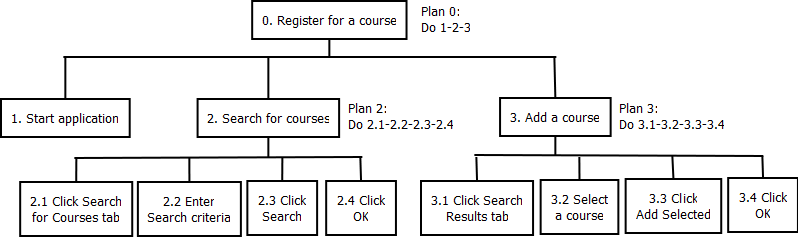
\includegraphics[width=130mm]{05/images/hta}
\end{figure}

\paragraph{CTT (Concurrent Task Tree)} Podobný strom jako HTA, ale s operátory a symboly. Úloha přihlášení: vyplním uživatelské jméno a zároveň heslo, pak je mi umožněho se připojit.

\begin{figure}[h!]
\centering
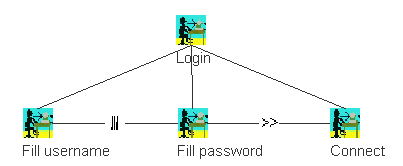
\includegraphics[width=100mm]{05/images/ctt}
\end{figure}
\vspace{-15px}
\begin{itemize}[itemsep=0px]
\item Enabling T1 $>>$ T2
\item Disabling T1 [> T2
\item Interruption T1 |> T2
\item Choice T1 [] T2
\item Iteration T1* nebor T1$_{n}$
\item Concurrency T1 ||| T2
\item Optionality [T]
\end{itemize}


\paragraph{Storyboard} Série snímků a skečů (\uv{komiks} popisující nějakou úlohu).

\paragraph{Scénáře} Jednoduché výpravné příběhy průběhu úkolu

\textit{\uv{Uživatel napíše všechny účastníky akce, vyplní místo a datum konání. Systém poté zkontroluje zda je vše vyplněno v pořádku a vytvoří událost.}}.

\paragraph{Případy užití} Popis interakce člověka se systémem..

\paragraph{Keystroke-Level Model (KLM)}
Cílem je vypočítat čas potřebný pro provedení úlohy
Operátory:
\begin{itemize}[itemsep=0px]
\item stisk klávesy (\textbf{K}eystroke) - určený rychlostí psaní
\item ukázat na cíl na displeji (\textbf{P}ointing) - určeno pomocí Fitt's Law
\item položit ruku na vstupní zařízení (\textbf{H}oming) - odhad měřením
\item mentální příprava akce (\textbf{M}ental preparation) - odhad měřením, heuristika pro předřazení
\item čas reakce systému (\textbf{R}eaction)
\end{itemize}
Jsou časové odhady (tabulkové) pro každý operátor. Předpokládá provádění úloh bez chyby, předpovídá jen efektivitu, ignoruje paralelní zpracování, prokládání úloh, mentální zátěž, plánování a řešení úlohy (\uv{přemýšlecí} čas, uvažovány jsou jen holé akce)


\paragraph{Goals, Operators, Methods, Selection Rules (GOMS)}
Nejznámější používaná metoda. Složky:
\begin{itemize}[itemsep=0px]
\item \textbf{Goals} - cíle z hlediska úmyslů koncového uživatele
\item  \textbf{Operators} - elementární perceptuální, kognitivní a motorické akce s fixním časem
bez ohledu na kontext
\item \textbf{Methods} - posloupnost operátorů a podcílů
\item \textbf{Selection rules} - if-then pravidla určující, kterou metodu použít
\end{itemize}

Předpokládá provádění úloh bez chyby, úlohy musí mít přesně definovaný cíl, nemodeluje proces řešení problému, chování uživatele

\paragraph{Dialog modeling}
Z HTA máme představu o posloupnosti kroků, potřebujeme popsat, jak při provádění kroků spolu budou komunikovat uživatel a počítač - jak bude probíhat dialog
\begin{itemize}[itemsep=0px]
\item textové (gramatiky, produkční pravidla, událostní algebry)
\item diagramy - (STN, PN, flowcharts, JSD)
\end{itemize}

\paragraph{State Transition Networks (STN)}
Varianta konečných automatů, konečný počet stavů a přechodů mezi nimi, automat se nachází v pravě jednom stavu (stavy jsou disjunktní). Reakcí na každý uživatelský vstup je přechod z daného stavu do nového stavu. Stav má přiřazenou akci, musí být odlišitelný od jiných stavů, charakterizován vstupy, které k němu vedou. Přechod mezi stavy může být vázán podmínkou, lze k nim přiřazovat popis akcí.
\begin{itemize}[itemsep=0px]
\item[$+$] model UI, se kterým lze experimentovat
\item[$+$] možnost automatického nebo poloautomatického vytváření UI
\item[$+$] kontrola vlastností (úplnost, reversibilita, dostupnost, nebezpečné stavy - ukončení bez uložení)
\item[$-$] některá zařízení mohou mít velká množství stavů
\end{itemize}

\begin{figure}[h!]
\centering
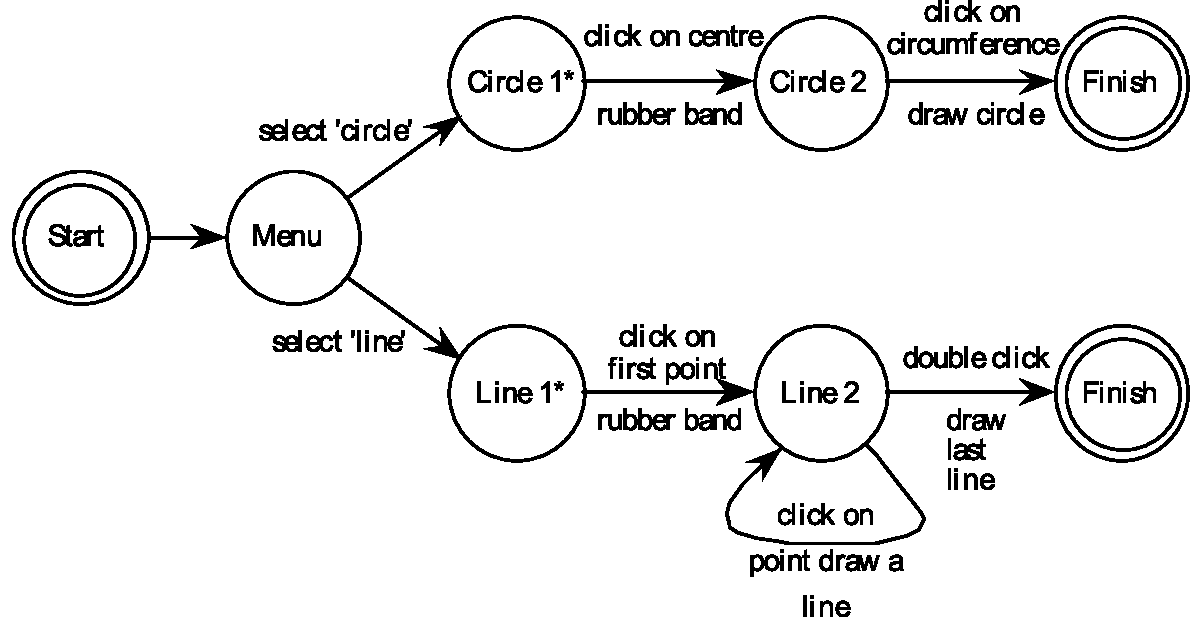
\includegraphics[width=130mm]{05/images/stn}
\end{figure}

\textbf{hierarchické STN} - varianta pro popis složitých dialogů, obsahuje sub-dialogy (vnořené další sítě).

\paragraph{Petriho sítě (PN)} Oproti STN mají synchronizaci - pokračování při splněné podmínce % NUR
    %!TEX root=../oi-magistr-si.tex
\section[NUR - Prototypování uživatelských rozhraní]{Prototypování uživatelských rozhraní}
Prototypování se dělá v ranných fázích návrhu. Rozděluje na \textbf{Low-Fidelity} a \textbf{High-Fidelity} prototypování.

\subsection{Low-Fidelity}
První náčrtky rozhraní. Jsou to víceméně narychlo načmárané skicy bez detailů, spiše jde o základní rozvržení (layout) prvků, žádná interakce. Typicky skicy na papíru nebo na elektronických prototypovacích SW (není na finálním zařízení). Je to spíše o rychlém zhodnocení nápadů, které jsou převedeny na papírový prototyp.

\begin{itemize}[itemsep=0px]
\item velké množství nápadů/alternativ
\item krátká doba vývoje - hodiny/dny
\item neběží na finálním zařízení
\item bez interakce
\item testování v laboratoři
\end{itemize}

\vspace{20px}

\begin{figure}[h!]
\centering
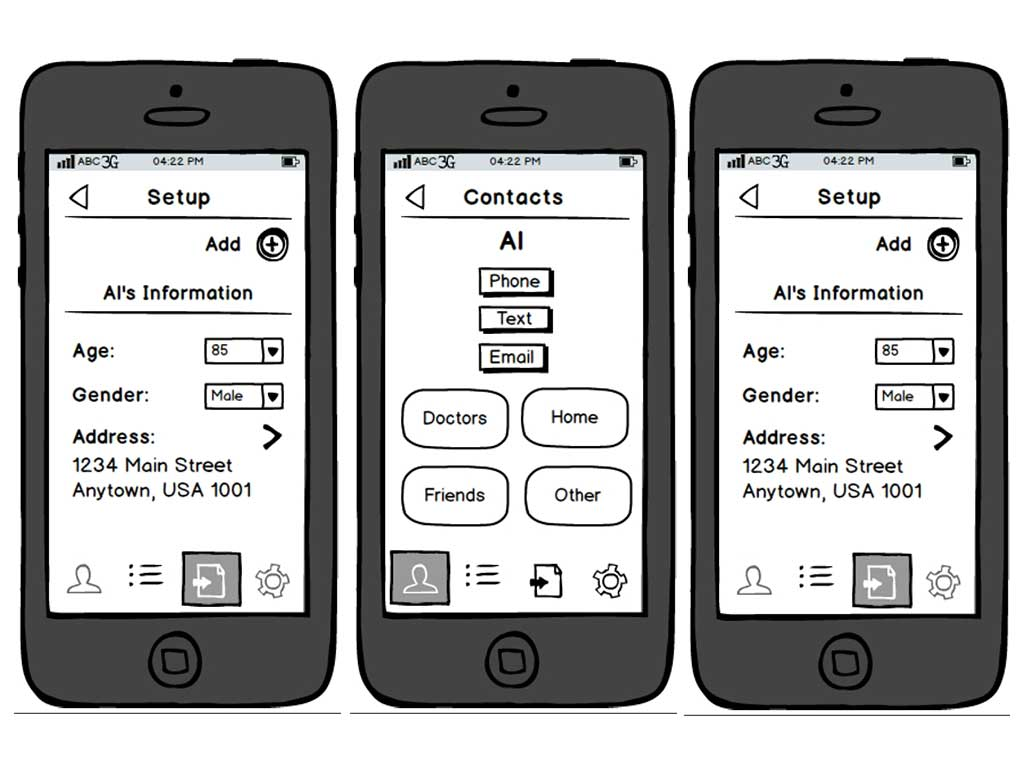
\includegraphics[width=110mm]{06/images/lofi}
\end{figure}

\vspace{20px}

Např. prototypování mobilní app. Vytvoří se několik papírků, každý popisuje krok aplikace. Interakce v podobě fiktvního klikání na papír, dochází k výměně papírků (změna stavu) a tím dochází k fiktivní interakci.

\subsection{High-Fidelity}
Iluze finálního vizuálního (i interagujícího) návrhu. Vzhled by měl následovat \textit{guidelines} cílové platformy (MS Windows, Android, iOS, ..). Prototyp již ve funkční podobě na cílovém zařízení, např. na telefonu. Interakce realizována jakoby to byla již výsledná aplikace, ovšem logika ještě nemusí být implementována (dummy data, \textit{Wizard of Oz}, atd.,). Hlavní části

\begin{itemize}[itemsep=0px]
\item málo alternativ (pokud vůbec nějaké jsou)
\item dlouhá doba vývoje - dny/týdny
\item dostupné na finálním zařízení
\item podoba a interakce téměr podobná té finální
\item testování v laboratoři a v \uv{terénu} (v reálných podmínkách využití)
\end{itemize}

\begin{figure}[h!]
\centering
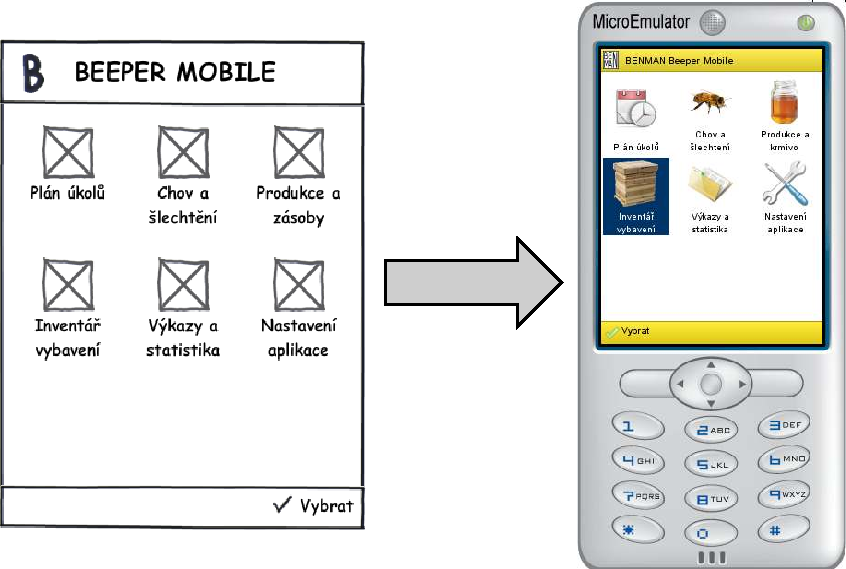
\includegraphics[width=80mm]{06/images/hifi}
\end{figure}

\paragraph{Problémy s prototypováním}
\begin{itemize}[itemsep=0px]
\item U lo-fi prototypů dochází ke skipování hlubokých (detailních) uživatelských požadavků
\item user confusion: hi-fi prototyp vs. finální aplikace
\item drahé a žrout času (speciálně hi-fi)
\end{itemize} % NUR
    %!TEX root=../oi-magistr-si.tex
\section[OSP - Open source,git,lincence]{Techniky správy a organizace rozsáhlých softwarových projektů. Nástroje pro správu verzí zdrojových kódů, sledování chyb, pro automatické generování dokumentace a podporu orientace v rozsáhlých projektech. Způsoby komunikace mezi vývojáři navzájem a i s uživateli. Systémy pro sledování a řešení chyb a uživatelskou podporu. Open-source licence a z nich vyplývající práva a licence. Postup začlenění úpravy (patche) do velkého open-source projektu (např. Linuxové jádro)}

\paragraph{Motivace pro verzování zdrojového kódu} Verzování kódu umožňuje sdílení kódu mezi vývojáři, zálohování, paralelní vývoj v několika souběžných větvích, vrácení se ke konkrétní revizi kódu, zjištění autorství nebo zobrazení statistik. Bez verzovacího systému není možná efektivní spolupráce více vývojářů na jednom projektu. Verzovací systém přináší výhody i v případě, že na projektu pracuje jediný vývojář.

\subsection{Nástroje pro správu verzí kódu}
GIT je distribuovaný SCM\footnote{Source Code Management} od Linuse Torvaldse. Každá working copy je zároveň repozitář, nezávislé na centrálním serveru. Spoustu operací jako merge, branch,... lokálně. Commity jsou hash celé historie vedoucí ke commitu. Nevýhoda: častější konflikty Subversion (SVN) je centrální SCM, ale rozšířený = dobré nástroje, GUI atd. Míň konfliktů, ale závislost na serveru. CVS podobné SVN ale starší, nevýhody: drahé branchování, problémy s Unicode, netrackuje přejmenovávání a mazání souborů.

\subsection{Nástroje pro sledování chyb (bug trackers)} Jsou nástroje (např. bugzilla), které sledují a soustřeďují nalezené chyby. Každá chyba má vypsaný svůj \textit{ticket}, ve kterém jsou veškeré informace k chybě: popis, priorita, reportující osoba, přiřazená osoba, návrh úpravy (např. v podobě patche).

\subsection{Nástroje pro automatické generování dokumentace}
Javadoc generuje HTML dokumentaci z komentářů v Java kódu, Doxygen je multijazykový generátor dokumentace z kódu, Enterprise Architect umí generovat UML diagramy z kódu.

\subsection{Systémy pro spolupráci mezi vývojáři}
GitHub je populární sociální platforma pro vývojáře na hosting a spolupráci open-source projektů založený na použítí Gitu, Trac je project management systém v Pythonu, který si můžete nasadit na vlastní server, obsahuje wiki, bug tracking, time management, etc. Spíše pro menší projekty. JIRA je SaaS systém podobný Tracu se spoustou pluginů, hodí se pro větší projekty.


\begin{itemize}[itemsep=0px]
\item Google Groups a podobné mailing listy mohou také sloužit k podpoře.
\item wiki stránky
\item fóra
\end{itemize}

\subsection{Licence}
Svobodný software je software, který respektuje svobodu svých uživatelů a poskytuje jim čtyři základní svobody, které svobodný software definují (publikace FSF 1986):

\begin{enumerate}[itemsep=0px]
\item svoboda používat program za jakýmkoliv účelem
\item svoboda zkoumat a upravovat program (předpokladem je přístup
ke zdrojovému kódu)
\item svoboda šířit původní verzi programu
\item svoboda šířit upravenou verzi programu
\end{enumerate}

\begin{itemize}[itemsep=0px]
\item \textbf{Komerční software} – licence daná smluvními podmínkami jež uživatel potvrzuje při nákupu SW
\item \textbf{Freeware} – zdarma, většinou bez zdrojových kódů, podmínky mohou omezovat další šíření, (komerční) použití, zkoumání
\item \textbf{Shareware} – jako freeware, ale specifikuje pro které druhy použití je nutné pořídit placenou verzi
\item \textbf{Permisivní} (akademické) licence (BSD, MIT) – povolují použití/integraci do komerčního SW, vyžadují jen uvádění autora/ů (to je i instituce)
\item \textbf{Copyleftové} (reciproční) licence (GPL, LGPL, MPL)
vyžadují zahrnutí uživatelů do okruhu oprávněných osob k právu nakládat s dílem (modifikovat ho a šířit za stejných podmínek)
\end{itemize}
\paragraph{Upozornění:} Definice open-source nevyžaduje \textit{copyleft}.

\subsubsection{BSD (Berkeley Software Distribution)}
BSD licence je licence pro svobodný software, mezi kterými je jednou z nejsvobodnějších. Umožňuje volné šíření licencovaného obsahu, přičemž vyžaduje pouze uvedení autora a informace o licenci, spolu s upozorněním na zřeknutí se odpovědnosti za dílo.

\subsubsection{MIT License}

Licence podobná BSD licenci umožňuje se software nakládat téměř libovolně (používat, kopírovat, modifikovat, slučovat, publikovat, distribuovat či prodávat), jedinou podmínkou je zahrnutí textu licence do všech kopií a odvozenin software.

\subsubsection{Apache License}
Stejné myšlenkové základy jako licence BSD a MIT. Výslovná zmínka možnosti šířit odvozená díla pod jinou kompatibilní licencí.

\subsubsection{GNU GPL (GNU General Public License)}

GPL je nejpopulárnějším a dobře známým příkladem silně copyleftové licence, která vyžaduje, aby byla odvozená díla dostupná pod toutéž licencí. 

GNU General Public License. Software šířený pod licencí GPL je možno volně používat, modifikovat i šířit, ale za předpokladu, že tento software bude šířen bezplatně (případně za distribuční náklady) s možností získat bezplatně zdrojové kódy. Toto opatření se týká nejen samotného softwaru, ale i softwaru, který je od něj odvozen. Na produkty šířené pod GPL se nevztahuje žádná záruka. Licence je schválená sdružením OSI a plně odpovídá Debian Free Software Guidelines.

V rámci této filosofie je řečeno, že poskytuje uživatelům počítačového programu práva svobodného softwaru a používá copyleft k zajištění, aby byly tyto svobody ochráněny, i když je dílo změněno nebo k něčemu přidáno. Toto je rozdíl oproti permisivním licencím svobodného softwaru, jejímž typickým případem jsou BSD licence

\subsubsection{GNU LGPL (GNU Lesser General Public License)}

Lesser/Library GPL. Licence je kompatibilní s licencí GPL. Pod touto licencí se šíří zejména knihovny, protože narozdíl od licence GPL umožňuje nalinkování LGPL knihovny i do programu, který není šířen pod GPL.

\subsubsection{MPL (Mozilla Public License)}
Mozilla Public License. Základním elementem pokrytým licencí je každý jednotlivý zdrojový soubor. Autor takového souboru umožňuje komukoliv používat, měnit a distribuovat jeho zdrojový kód (i jako součást většího díla). Každá změna původních souborů je krytá licencí, tzn. musí se tedy zveřejnit. To samé platí pokud přenesete část původního souboru do nového souboru, tj. celý nový soubor je pak nezbytné zveřejnit. Pokud vytváříte nový produkt přidáním nových souborů, můžete pro tyto nové soubory použít libovolnou licenci. Binární verze lze licencovat libovolně, pokud to není výslovně v rozporu s MPL (zákaz distribuce zdrojů). Produkty pod touto licencí jsou distribuované jak jsou ("as is"), tj. bez záruk libovolného druhu.

\subsubsection{CreativeCommons}
Je license vhodná pro jakýkoli obsah, nejenom pro software. Do license si člověk může dát 1-4 z těchto atributů:
\begin{itemize}[itemsep=0px]
\item Attribution - nutno uvést autora originálního projektu
\item Noncommercial - možno upravovat jenom pro nekomerční účely
\item NoDerivatives - možno pouze kopírovat dané dílo, ale nikoliv ho upravovat
\item Share-alike - znamená virální copyleft
\end{itemize}


\subsection{Kontribuce do projektu}
TODO
% http://git-scm.com/book/cs/v1/Distribuovaný-charakter-systému-Git-Přisp%C3%ADván%C3%AD-do-projektu
 % OSP

    \bibliographystyle{_lib/csplainnat}
    {
        \footnotesize
        \def\CS{$\cal C\kern-0.1667em\lower.5ex\hbox{$\cal S$}\kern-0.075em $}
        \bibliography{reference}
    }

\end{document}
